\vspace{-.15cm}
\section{Related Work}

\begin{figure}
    \centering
    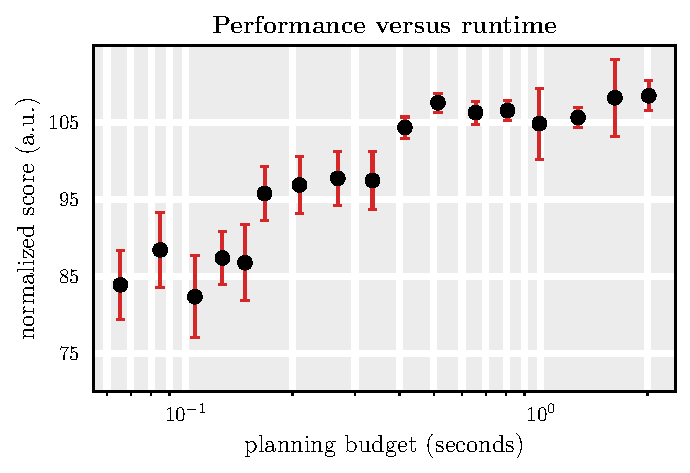
\includegraphics[width=\columnwidth]{images/speed.pdf}
    \vspace{-.25cm}
    \caption{
    % \small
    \textbf{(Fast Planning)}
    Performance of \method on Walker2d Medium-Expert when varying the number of diffusion steps to warm-start planning.
    Performance suffers only minimally even when using one-tenth the number of diffusion steps, as long as plans are initialized from the previous timestep's plan.}
    \label{fig:speed}
    \vspace{-5pt}
\end{figure}

Advances in deep generative modeling have recently made inroads into model-based reinforcement learning, with multiple lines of work exploring dynamics models parameterized as
convolutional U-networks \cite{kaiser2019mbatari},
stochastic recurrent networks \cite{ke2018modeling,hafner2018planet,ha2018worldmodels},
vector-quantized autoencoders \cite{hafner2021mastering,ozair2021vector},
neural ODEs \cite{du2020ode},
normalizing flows \cite{rhinehart2020imitative,janner2020gamma},
generative adversarial networks \cite{eysenbach2021mismatched},
energy-based models (\emph{EBMs}; \citealt{du2019model}),
graph neural networks  \cite{sanchez-gonzalez2018graph},
neural radiance fields \cite{li2021scene},
and Transformers \citep{janner2021sequence,chen2021transdreamer}.
Further, \citealt{lambert2020learning} have studied non-autoregressive trajectory-level dynamics models for long-horizon prediction.
These investigations generally assume an abstraction barrier between the model and planner.
Specifically, the role of learning is relegated to approximating environment dynamics; once learning is complete the model may be inserted into any of a variety of planning \cite{botev2013cem,grady2015mppi} or policy optimization \cite{sutton1990dyna,wang2019benchmarking} algorithms because the form of the planner does not depend strongly on the form of the model.
Our goal is to break this abstraction barrier by designing a model and planning algorithm that are trained alongside one another,
resulting in a non-autoregressive trajectory-level model for which sampling and planning are nearly identical.

A number of parallel lines of work have studied how to break the abstraction barrier between model learning and planning in different ways.
Approaches include training an autoregressive latent-space model for reward prediction \citep{tamar2016vin, oh2017vpn,schrittwieser2019muzero}; weighing model training objectives by state values \citep{farahmand2017valueaware}; and applying collocation techniques to learned single-step energies \citep{du2019model, rybkin2021model}.
In contrast, our method plans by modeling and generating all timesteps of a trajectory concurrently, instead of autoregressively, and conditioning the sampled trajectories with auxiliary guidance functions.

% A number of parallel lines of work have integrated model learning and planning. Approaches include learning latent spaces for planning using rewards \citep{tamar2016vin, oh2017vpn,schrittwieser2019muzero, farahmand2017valueaware};
% combining state, reward, and value prediction into a single model \citep{janner2021sequence}; and applying trajectory optimization to learned models  \citep{du2019model, rybkin2021model}.
% In contrast, we train a probabilistic model for trajectory optimization and plan by composing auxiliary cost guidance functions and user-specified constraints.

Diffusion models have emerged as a promising class of generative model that formulates the data-generating process as an iterative denoising procedure \citep{sohldickstein2015nonequilibrium, ho2020denoising}.
The denoising procedure can be seen as parameterizing the gradients of the data distribution \citep{song2019generative}, connecting diffusion models to score matching \cite{hyvarinen2005score} and EBMs \citep{lecun06atutorial, du2019implicit, nijkamp2019learning,grathwohl2020stein}.
Iterative, gradient-based sampling lends itself towards flexible conditioning \citep{dhariwal2021diffusion} and compositionality \citep{du2020compositional}, which we use to recover effective behaviors from heterogeneous datasets and plan for reward functions unseen during training.
While diffusion models have been developed for the generation of images \cite{song2020denoising}, waveforms \cite{chen2020wavegrad}, 3D shapes \cite{zhou2021shape}, and text \cite{austin2021structured}, to the best of our knowledge they have not previously been used in the context of reinforcement learning or decision-making.